\chapter{Btrw - Job Submission \& Editing Tool}
\label{chp:btrw}

\includegraphics{img/win3.png} 

\progname{Btrw} can be used to create and edit saved job files on the PC hard disk and submit
them to a server running \ProductName{} for execution.

Job files saved using the \textbf{Unqueue} command in \progname{btqw} are in the same format
as understood by \progname{btrw}.

Unlike the Visual C++ version of the Windows clients, jobs are saved as a single XML file rather
than a command file and a job file.

Jobs may be submitted to any of the servers set up under the server list of \progname{btqw}. The servers
must be online, but they need not be connected under \progname{btqw}.

\section{Mode of operation}

\progname{Btrw} displays a list of opened job files. This list is saved when \progname{btrw} exits, and reloaded when
it is restarted.

New jobs may be created with attributes set up from a list of default attributes which can be set up and adjusted from a
separate menu entry.

Any of the jobs may be selected, edited, saved and submitted to a server running \ProductName.

\section{The Main Window}
When \progname{btrw} is invoked for the first time the main window will be displayed, looking something like this:

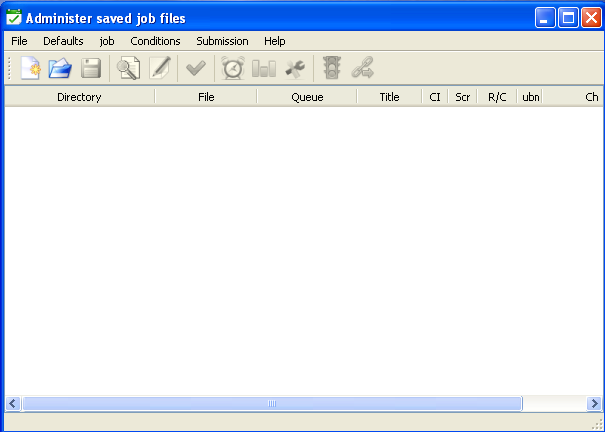
\includegraphics{img/btrwinitscr.png}

The main screen is divided into two key functional areas. The top area
contains menus and short cut buttons for issuing commands. The bottom
is used to display a list of the job files which \progname{btrw} currently
has open.

Wherever possible,
\progname{Btrw} uses similar windows and dialogs to \progname{btqw} for specifying the job options.

To edit job scripts \progname{btrw} has its own internal editor or it can invokes an editor of the
user's choice.

\section{The Menus and Shortcut Buttons}
All commands are performed by selecting a menu option or clicking on the
equivalent shortcut button. Some of the menu options may also be
selected using shortcut keys, which are indicated to the right of the
relevant options in each menu.

\subsection{File Menu}
The file menu provides options for creating, opening and saving jobs and also for configuring \progname{btrw} and quitting.

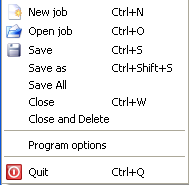
\includegraphics{img/btrwfilemenu.png}

\textbf{New Job} creates a new job, using the current default settings \textit{(although you should
be careful to set these up first)} ready for editing.

\textbf{Open job} opens a previously created job file. This might have been created by a previous run of \progname{btrw}
or via the \textbf{Unqueue} command in \progname{btqw}.

\textbf{Save} saves the currently-selected job and attributes to file, prompting for a file name and directory
if necessary.

\textbf{Save As} saves the currently-selected job and attributes to a new file.

\textbf{Save All} saves to file all the jobs which have been edited and have unsaved changes.

\textbf{Close} closes the currently-selected job file and removes it from the displayed list.

\textbf{Close and Delete} closes the currently-selected job file, removes it from the displayed list and also deletes the file.

\textbf{Program Options} \label{bkm:progopts}displays a dialog to modify the overall options used by \progname{btrw}.

\textbf{Quit} exits the program.

The following shortcut buttons are provided on the toolbar.

\begin{tabular}{l p{12cm}}

\includegraphics{img/btrwnewjob.png} & Is a shortcut for \textbf{New Job}\\

\includegraphics{img/btrwopenjob.png} & Is a shortcut for \textbf{Open Job}\\

\includegraphics{img/btrwsavejob.png} & Is a shortcut for \textbf{Save}\\
\end{tabular}

\subsection{The Defaults Menu}
The defaults menu provides a set of preset options which are applied to all new jobs
which are subsequently created.

It is probably a good idea to set up options appropriate to your environment before
starting to create any new jobs.

(Note that default conditions and assignments are provided for on the \textbf{Conditions} menu.)

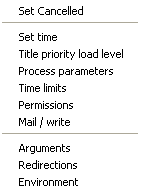
\includegraphics{img/btrwdefsmenu.png} 

\textbf{Set Cancelled} (a tick appears next to it if this is selected) sets the cancelled state as the default for new jobs.

\textbf{Set time} Sets a default set of time and repeat parameters (note that this is separate from the \textbf{Time defaults} option
in \progname{btqw}).

\textbf{Title priority load level} Sets default values for title, priority, load level and command interpreter.

\textbf{Process parameters} Sets default values for the
process parameters: working directory, ulimit, umask, exit code ranges,
advance time on error flag.

\textbf{Time limits} Sets default values for detecting and stopping over-running jobs.

\textbf{Permissions} Sets default values for job access modes (these are initialised to the user's default values on the default server).

\textbf{Mail / Write} Sets default values for the job completion flags.

\textbf{Arguments} Sets default values for job arguments.

\textbf{Redirections} Sets default values for job I/O redirections.

\textbf{Environment} Sets default values for environment variables.

\subsection{Job Menu}
The job menu provides options for setting various attributes of the currently-selected job file.

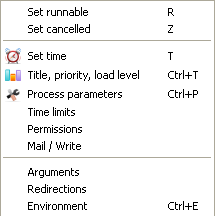
\includegraphics{img/btrwjobmenu.png} 

\textbf{Set runnable} sets the job so that if submitted, it is ready to run immediately (if the conditions
and time constraints are met).

\textbf{Set cancelled} sets the job so that if submitted, it will be in ``cancelled'' state, i.e. held until
set ready to run by the operator.

\textbf{Set time} brings up a dialog to set the time and repeat options for the job.

\textbf{Title, priority, load level} brings up a dialog to set the title, priority, load level and command
interpreter for the job.

\textbf{Process parameters} brings up a dialog to set the process parameters i.e. working directory, umask,
ulimit, exit code ranges and export settings.

\textbf{Time limits} brings up a dialog to set the running time constraints for the job.

\textbf{Permissions} brings up a dialog to set the modes or access permissions for the job.

\textbf{Mail/Write} brings up a dialog to set the notification flags for the job.

\textbf{Arguments} brings up a dialog to set the arguments for the job.

\textbf{Redirections} brings up a dialog to set the I/O redirections for the job.

\textbf{Environment} brings up a dialog to set the environment for the job.

The following shortcut buttons are provided on the toolbar.

\begin{tabular}{l p{12cm}}

\includegraphics{img/btqwtimeset.png} & Set time\\

\includegraphics{img/btqwtitprill.png} & Title, priority, load level\\

\includegraphics{img/btqwprocpar.png} & Process parameters\\
\end{tabular}

\subsection{Conditions menu}
The conditions menu provides options for setting conditions and assignments together with
default sets of conditions and assignments to apply to new jobs.

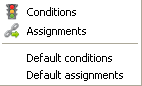
\includegraphics{img/btrwcondmenu.png} 

\textbf{Conditions} brings up a dialog to set or edit the conditions on the currently-selected job.

\textbf{Assignments} brings up a dialog to set or edit the assignments on the currently-selected job.

\textbf{Default conditions} brings up a dialog to set or edit the default conditions to be applied to any
newly created job.

\textbf{Default assignments} brings up a dialog to set or edit the default assignments to be applied to any
newly created job.

The following shortcut buttons are provided on the toolbar.

\begin{tabular}{l p{12cm}}

\includegraphics{img/btqwcond.png} & Is a shortcut for \textbf{Conditions}\\

\includegraphics{img/btqwass.png} & Is a shortcut for \textbf{Assignments}\\
\end{tabular}

\subsection{Submission Menu}
This menu provides options for submission of jobs and for viewing and/or editing the job script.

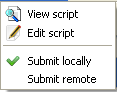
\includegraphics{img/btrwsubmenu.png} 

\textbf{View script} displays the script of the job in a window. Any number of job scripts may be displayed in this way.

\textbf{Edit script} creates an initial script if none is provided and displays it for editing. If the program option
to set an external editor is provided in program options (see page \pageref{bkm:progopts}) then this is used, otherwise
an internal editor is used.

\textbf{Submit locally} submits the job to the queue on the server marked under the program options (see page \pageref{bkm:progopts}) as
the default server.

\textbf{Submit remote} prompts for a server and submits the job to the queue on that server. (Note that some of the settings and
permissions are assumed to be the same as those for the default server).

The following shortcut buttons are provided on the toolbar.

\begin{tabular}{l p{12cm}}

\includegraphics{img/btqwviewjob.png} & Is a shortcut for \textbf{View script}\\

\includegraphics{img/btrwjobedit.png} & Is a shortcut for \textbf{Edit script}\\

\includegraphics{img/btrwjobsubmit.png} & Is a shortcut for \textbf{Submit locally}\\
\end{tabular}

\subsection{The Help Menu}
Help for using \progname{btrw}.


\includegraphics{img/btrwhelpmenu.png} 

\textbf{About} displays information, such as release number, about the
version of \progname{btrw} that is running.

\subsection{Right-click menu}
Right-clicking on a line on the \progname{btrw} display brings up the following commonly-used
options:

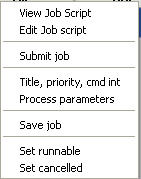
\includegraphics{img/btrwpopup.png}

\textbf{View Job Script} displays the script of the selected job.

\textbf{Edit Job Script} brings up an editor window to edit the script of the selected job.

\textbf{Submit job} submits the job to the main server as selected under \textbf{Program Options}.

\textbf{Title, priority, cmd int} and \textbf{Process parameters} are equivalent to the corresponding menu selections
on the main menu.

\textbf{Save job} saves the job to file.

\textbf{Set runnable} and \textbf{Set cancelled} select the same options as for the job menu selections.

\section{Creating a New Job}
Creating a new job is hopefully a lot easier than with the Visual C++
version of the Windows clients, notably because only one file is used to
hold the job and the job script.

This section is intended to give an overview of how this is done, all the
way to submitting the job.

\subsection{Checking program options}

At least the first time you attempt to create a job, you should review
the program options to select the preferred server (from which default
permissions will be taken).

Use the \textbf{File - Program options} menu item to get the dialog:

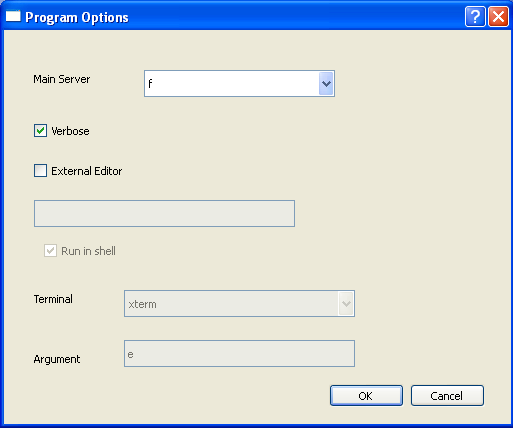
\includegraphics{img/btrwpoptsdlg.png}

The first entry is the main server, where servers set up in \progname{btqw}
are listed. Select the required one using the drop-down box.

Note that this server does not have to be one to which \progname{btqw} usually
communicates.

The \textbf{Verbose} checkbox is used to cause the job number of jobs successfully
submitted to be displayed in a pop-up box. Set this as required, but probably
you will wish to.

The \textbf{External Editor} selection allows you to edit job scripts other than
with the internal editor. However we do not particularly recommend this. It is
mostly intended for use when the program is run on UNIX-style systems.

\subsection{Checking the default settings}

At least the first time you attempt to create a job, you may probably want
to review the default settings.

If you first select {Defaults - Process parameters}, the following dialog should be
displayed.

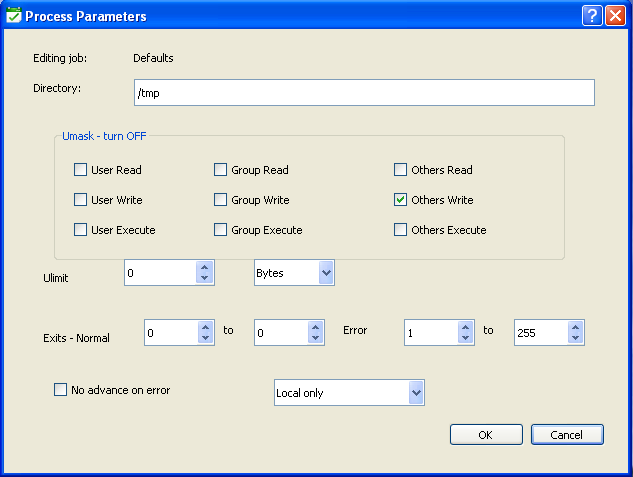
\includegraphics{img/btrwdefppdlg.png}

The default working directory is initialised to \filename{/tmp}. This should probably be
changed to a more appropriate working directory. Remember that environment variables
and constructs of the form \exampletext{~user/batchdir} are expanded here so you could
put some appropriate generic construct in here.

Another aspect to consider is the export settings. By default this is set to
\textit{local only}, so that jobs are only visible on the server itself. You may
wish to set this to \textit{Exported} so that the jobs created are at least visible
with \progname{btrw}.

You may want to consider resetting some of the other options in the default section, perhaps by
setting a convenient prefix to titles to be adjusted later.

\subsection{Creating a new job}

To actually create the new job, either select \textbf{File - New Job}, use the toolbar shortcut

\includegraphics{img/btrwnewjob.png} or use the keyboard shortcut \textit{ctrl+N}.

The new job is created, copying in initial values from the defaults, and the screen display should then
look like this:

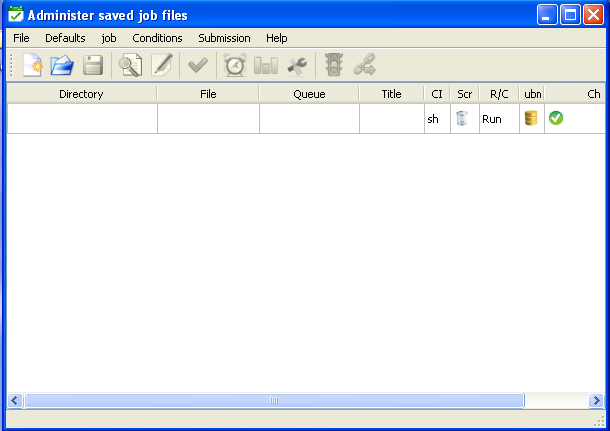
\includegraphics{img/btrwnewjob1.png}

The directory and file columns refer to the location on the Windows client, not to anything
referred to in the job, so these are empty to start with. If the job has a title, this is displayed
in the relevant column. The name of the command interpreter is also displayed.

The next 4 columns show the state of the job.

\begin{enumerate}
\item The first of these column shows whether a script has been created for the job. All jobs should have
a script. If the job has a script then 
\includegraphics{img/hasscript.png} is displayed, otherwise

\includegraphics{img/noscript.png} is displayed.

\item The second of the columns indicates whether the job will be submitted in ``cancelled'' state or
ready to run state.

\item The third of the columns indicates whether the job has been submitted in its current form. It will
be 
\includegraphics{img/submitted.png} if it has been and there are no changes since, otherwise it
will be 
\includegraphics{img/unsubmitted.png}.

\item The final column indicates whether there are unsaved changes. If there are none (including a new
job identical to the default) then 
\includegraphics{img/saved.png} is displayed, otherwise

\includegraphics{img/changed.png}.
\end{enumerate}

Next perhaps give it a title by selecting the job and the menu entry \textbf{Job - Title, priority, load level}
or the 
\includegraphics{img/btqwtitprill.png} button.

This should display a dialog such as the following:

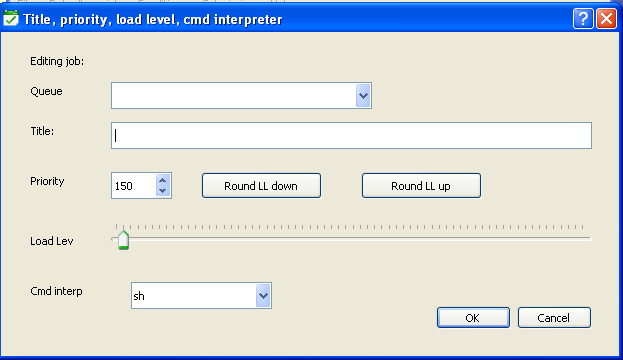
\includegraphics{img/btrwnewjob2.png}

Type in a title, perhaps \filename{Example} and possibly adjust the command interpreter, priority and load level.

Note that a queue prefix may be automatically prepended to the title, with prefixes previously encountered available from
the drop-down box.

Note that the priority may only be adjusted between limits set for your user name. Likewise the load level may be restricted
to only that set for the command interpreter selected, in which case the buttons and slider may be disabled.

The ``round up'' and ``round down'' buttons are used to adjust the load level to tidy multiples of ten.

After the title has been set and the OK button pressed the display should look like this:

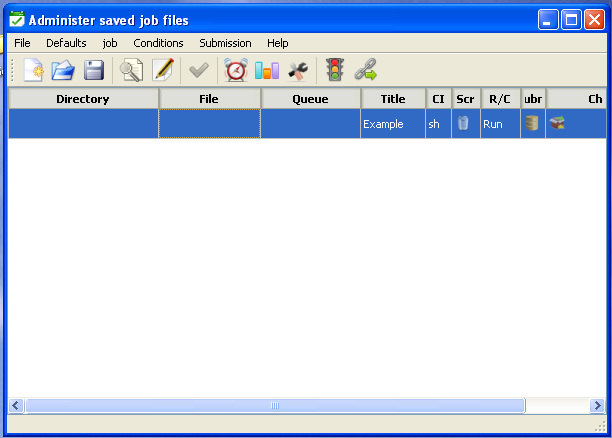
\includegraphics{img/btrwnewjob3.png}

The icon on the end has changed to indicate that the job has unsaved changes and the title
has been inserted.

Next set up a script for the job by selecting \textbf{Edit script}.

This should bring up a window showing the job title and command interpreter name.

Scripts are assumed to be text files. Note that prefixes such as \exampletext{\#! /bin/sh} are not required.

When done, the icon in the ``has script'' column will be appropriately changed.

You may want to save the job at this point to a file on the PC. This brings up a standard
Windows-style save box. When done, the display will change to

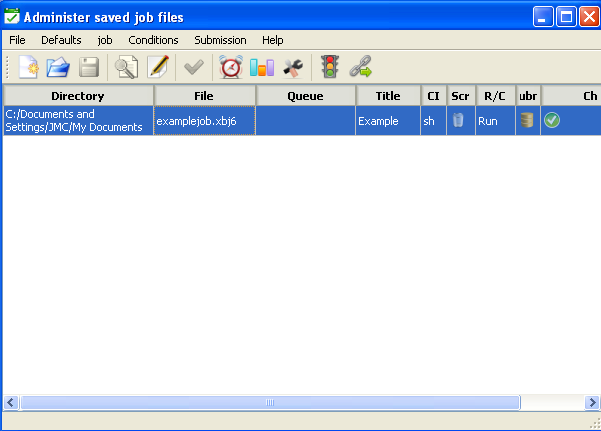
\includegraphics{img/btrwnewjob4.png}

The directory and file names on the PC are filled in and the final column is changed to indicate that there are no unsaved changes.

Finally submit the job to the main server by using the 
\includegraphics{img/btrwjobsubmit.png} button or equivalents.

If all goes OK and the \textbf{Verbose} option was set in program options, the message:

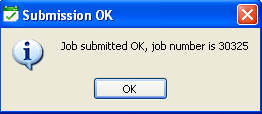
\includegraphics{img/btrwnewjob5.png}

The icon against the job will be changed to indicate that the job has been submitted on the main display.


